\graphicspath{ {Context/Images/} }


\chapter{Electronic Health Records Analytics}
\label{cha:context}

\section{Introduction}

In section \ref{sec:ehr} we explain what electronic health records are and how these are represented. In section \ref{sec:ehra}, we explain how the electronic health records can be used to retrieve useful medical information. We also explain different approaches to retrieve this information from the health records. Those approaches range from querying databases to more advanced machine learning techniques. After stating the general context we are working in and what we want to improve, we state the outline of information in the thesis in section \ref{sec:outline}.


\section{Electronic Health Records}
\label{sec:ehr}

An electronic health record (EHR) is a collection of time-stamped data about a patient over a period point of time. It is stored digitally and thus can be established for a large number of patients over a long time period. \\
The data stored in an EHR provides an overview of the patients' health information. Health information like demographics, medical history, diagnoses, medications, and such, are stored \cite{HealthIT:online}. \\

Recently large countries like the US and the UK, are each investing more than $20$ billion dollars into EHR systems \cite{EHRworld:article}. Those systems are adopted by around $70$\% of the physicians in the US, but of those systems a lot of different implementation are used. Which means a large number of physicians are using different methods or systems. This causes different ways of information representation and makes it harder to compare EHRs across different systems. We focus on disease codes in the next section and introduce two standards: one used by mainly insurance companies and the other used by pharmaceutical companies. 


\subsection{Disease Codes}

To make EHRs practical it is important to adhere to standards for data formatting. A well-documented and consistently used standard makes it easy to store and extract information from large-scale databases of EHRs. Without the possibility of extracting information, an EHR becomes a simple digital version of medical records on paper. \\
Part of an EHR consists of the diagnosis of the patient. It provides information about his disease trajectory and allows analysis on his health situation. With a uniform system for classifying diseases nationwide, it is possible to provide a general picture on health situations of populations. Several have been defined and their usage is scattered. We discuss the $2$ most relevant to our work.

\subsubsection{ICD-10}

The International Statistical Classification of Diseases and Related Health Problems (ICD) is a medical classification list made by the World Health Organization (WHO) \cite{WHO_ICD:online}. Several variants are available like ICD-9, ICD-10, ICD-10 CM, and others. The ICD-10 contains more than $14,400$ codes about diseases, disorders, injuries, and other related health conditions. For example, the code for a sprained ankle is $S93.4$. It also provides hierarchical categories for those codes to allow a more general overview of diseases. ICD is mainly used by insurance companies.


\subsubsection{MedDRA}

The Medical Dictionary for Regulatory Activities (MedDRA) provides medical terminology in the form of disease codes \cite{MedDRA:online}. A MedDRA code is an eight digit numeric code where the code itself has no meaning. The code functions as an unique identifier so new terms are just identified with the next available code. Note that this system does not provide a clear and easy to use system to retrieve a hierarchical structure of a code. MedDRA is mainly used by pharmaceutical companies.

\section{EHR Analytics}
\label{sec:ehra}

EHRs provide a massive amount of data which in principle can be used to create useful insights. The data contains the medical history of a patient including medical measurements, diagnoses, prescribed drugs, and demographics (see figure \ref{fig:matrixPatient}, where procedures (CPTs), lab results (LABs), visits to primary care physician (PCP) and visits to specialists (SPEC) are part of the EHR). Based on those values, we could obtain the following insights:

\begin{itemize}

\item Effects of drugs
\item Medical costs for certain diseases
\item Duration and recovery percentage of certain diseases
\item Correlation between demographics and certain diseases
\item Link between current health state and health history
\item Classification and prediction of future health states based on history

\end{itemize}

Those insights can be offered on an individual level, which means a right intervention to the right patient at the right time. EHR analytics can be used to have a personalized care and benefits the healthcare system by cutting costs and improve outcomes \cite{rand1:article}. \\

EHR analytics is an active research field as a lot of different problems need to be solved, like different codings, privacy, interpretation, and large amounts of data. In the following sections we talk about current EHR analytical methods.


\subsection{Querying}

Analytics in epidemiology on EHRs is typically done through querying a database \cite{EHRquery:journal}. A specialist has a hypothesis about correlations between conditions or patients. He can support this idea by selecting cases in EHRs and analyzing the results of his query. \\
This method is based on the knowledge and experience of a specialist. The information has to be actively sought after and unexpected or complex correlations are not always considered. Some complex relations cannot be found because of the limitations of the querying language, ex. a first-order logic query language. Currently The Health Improvement Network (THIN) research team at UCL conducts these kinds of research \cite{THIN:online}.

\subsection{Data Analytics}

More advanced methods are applied to EHRs than querying. In general, the goal is to find patterns in the EHR data which then can be used to predict outcomes of treatments or classify a patient's disease trajectory \cite{EHRbigdata:slides}. \\

Several predictive/classification methods from machine learning can be used and show promising results \cite{EHRmining:article}. Those results are achieved by using exploratory methods which are applied to the EHR data. We also note that methods in \cite{EHRmining:article} as Multi-layer Perceptron networks are not ideal for prediction of time-series like medical data, see section \ref{sec:PatientClassification}. We conclude that there is still a lot of room for improvement. \\
 
More specialized approaches are also applied to EHR data \cite{EHRrecommender:article} besides the above mentioned machine learning techniques. 
An EHR of a patient can be transformed into a matrix structure, see figure \ref{fig:matrixPatient}. On these matrix structures, large-scale data mining algorithms can be applied. Those make it possible to mine patterns in EHR data. The patterns found can be used as the basis for predictive models.

\begin{figure}[!htb]
	\centering
	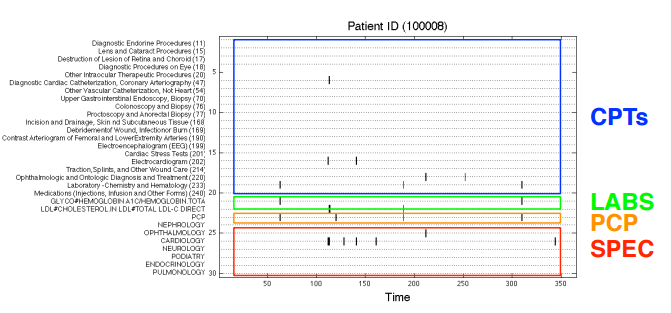
\includegraphics[width=\textwidth]{matrixPatient.png}
	\caption{Example of an EHR transformed into a matrix structure \cite{EHRrecommender:article}}
	\label{fig:matrixPatient}
\end{figure}

It is also possible to define patient similarities \cite{EHRsimilarity:article}. So when a patient is similar to a previous known case, his treatment can be based on those previous experiences. In a way, it could be seen as a similar approach as a recommender system \cite{recommender:article}.


\subsection{Data Mining}

In 2015, a more data mining approach is used to find patterns in EHR data on a dataset of the Danish population \cite{Brunak:article}. The results from \cite{Brunak:article} are clusters of disease trajectories which will be used to validate our approach described in chapter \ref{cha:background}. Their results are used because it is currently the largest study performed on EHRs. You can find an example of a clustered trajectory in figure \ref{fig:clusterGraphDanish}. \\

\begin{figure}[!htb]
	\centering
	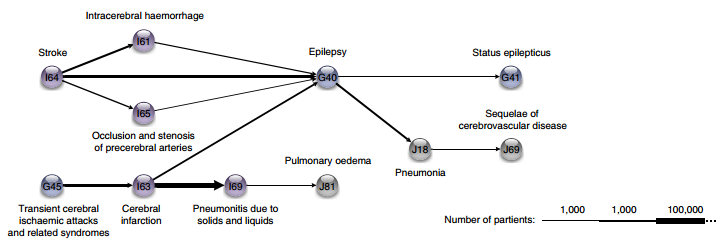
\includegraphics[width=\textwidth]{clusterGraphDanish.png}
	\caption{Cerebrovascular disease trajectory cluster for the Danish population \cite{Brunak:article}}
	\label{fig:clusterGraphDanish}
\end{figure}

The dataset which is used to apply the data analysis on, consist of EHRs collected over $15$ years on over $6$ million patients in Denmark. The size of this dataset makes it possible to retrieve statistically significant results. \\

They start with finding pairs of patients' diagnoses which have a strong temporal correlation between them. After finding the correlated pairs, a test for directionality is applied. From this, only the pairs with a high enough indication for a direction are kept, ie which often appear one after the other within a certain time span. \\

The directed pairs are then connected into longer trajectories when they have overlapping diagnoses. The found trajectories are then clustered. From the clusters, diagnoses can be found which are key in the disease progression. Those key diagnoses could be used to predict future disease progression of patients. 



\section{Outline}
\label{sec:outline}

In this chapter, we introduced you to the field of Electronic Health Record Analytics and some current research directions. We state this is an active research field with a lot of directions left to explore. \\
In chapter \ref{cha:background}, we start with introducing some terminology and general background knowledge needed to introduce our approach in the field of Electronic Health Record Analytics. Then we explain our own approach, namely generalized Word2Vec approaches, and how those can be applied on medical data. \\
In chapter \ref{cha:implementation}, we show the methods we used to implement our own approaches. This allows us to execute experiments and validate our approaches. \\
In chapter \ref{cha:conclusion}, we talk about conclusion we can take from this thesis and sum up the results we achieved. \\
The last chapter, namely chapter \ref{cha:futureWork}, we explore some possible improvements on our approaches and some future directions left to explore using our own approaches.


\section{Conclusion}

EHRs contain important information of a patients medical history and current state. When a large amount of EHRs is available, relevant results can be found in the form of patterns. Those pattern can be used to predict and improve medical outcomes on a personal level. \\
The methods we describe vary from simple to very complex. But there is still room for improvement, especially in the field of advanced machine learning algorithms. The results of the Danish paper can be used to have a first validation of our approach, namely a generalized Word2vec approach. \\

In the next chapter we explain the required background knowledge to understand our approach on finding patterns in EHRs. After introducing you to those concepts, we also explain our approach, namely a generalized Word2vec approach.


%%% Local Variables: 
%%% mode: latex
%%% TeX-master: "thesis"
%%% End: 
